\documentclass{article}

\usepackage{lipsum}
\usepackage{amsfonts}
\usepackage{amsmath}
\usepackage{amsthm}
\usepackage{graphicx}
\usepackage{epstopdf}
\usepackage{algorithmic}
\ifpdf%
  \DeclareGraphicsExtensions{.eps,.pdf,.png,.jpg}
\else
  \DeclareGraphicsExtensions{.eps}
\fi
\usepackage{amsopn}
\DeclareMathOperator{\diag}{diag}
\usepackage{booktabs}
\usepackage{bbm}
\usepackage{bm}
\usepackage{caption}
\usepackage{subcaption}
\usepackage[utf8]{inputenc}
\usepackage[T1]{fontenc}
\usepackage[margin=1.5in]{geometry}
\usepackage{hyperref}

\newcommand{\norm}[1]{\left\lVert#1\right\rVert}
\newcommand{\normtwo}[1]{\left\lVert#1\right\rVert_2}
\newcommand{\abs}[1]{\left\lvert#1\right\rvert}
\newcommand{\mat}[1]{\bm{{#1}}}
\renewcommand{\vec}[1]{\bm{{#1}}}
\newcommand{\lequiv}{\Leftrightarrow}
\newcommand{\bigO}[1]{\mathcal{O}\!\left(#1\right)}
\newcommand{\ceil}[1]{\left\lceil #1 \right\rceil}
\newcommand{\floor}[1]{\left\lfloor #1 \right\rfloor}
\newcommand{\sfrac}[2]{#1/#2}
\newcommand{\hquad}{\enskip}
\newcommand{\expected}[1]{\mathbb{E}\left[#1\right]}
\newcommand{\mspan}[1]{\text{span}\left( #1 \right)}
\newcommand{\prob}[1]{P\left(#1\right)}
\newcommand{\probt}[1]{P\left( \text{#1} \right)}
\newcommand{\condprob}[2]{P\left(#1 \:|\: #2\right)}
\newcommand{\condprobt}[2]{P\left(\text{#1} \:|\: \text{#2}\right)}
\newcommand{\bayes}[2]{\frac{\condprob{#2}{#1}\prob{#1}}{\prob{#2}}}
\newcommand{\bayesx}[3]{\frac{\condprob{#2}{#1}\prob{#1}}{\condprob{#2}{#1}\prob{#1} + \condprob{#2}{#3}\prob{#3}}}
\newcommand{\sech}{\text{sech}}
\newcommand*{\vertbar}{\rule[-1ex]{0.5pt}{2.5ex}}
\newcommand*{\horzbar}{\rule[.5ex]{2.5ex}{0.5pt}}
\newcommand{\vect}[2]{\underline{{#1}}_{{#2}}}
\newcommand{\basisp}[1]{\underline{{p}}_{{#1}}}
\newcommand{\basisq}[1]{\underline{{q}}_{{#1}}}
\newcommand{\coeff}[1]{\underline{{a}}_{{#1}}}
\newcommand{\bestfit}{\underline{\bar{x}}}
\newcommand{\grad}{\nabla}
\newcommand{\laplace}{\Delta}
\newcommand{\setbar}{\:\middle|\:}
\renewcommand{\div}{\grad \cdot}
\renewcommand{\Re}{\text{Re}}

\begin{document}
\section{Introduction}
Here, we are exploring the use of AMG methods for the \textit{unsteady Navier-Stokes} equations.  In particular, we are attempting to answer the following research questions:
\begin{enumerate}
\item If an algebraic multigrid method (AMG) is used in the numerical solution to the Navier-Stokes equations, are we able to learn anything (in a machine-learning sense) about the solver?  Particularly, which AMG setups are most convergent and which fail to solve the problem for a specific timestep?
\item If we do indeed learn something about the solver, can we use this to optimize and boost the solver efficiency (in terms of computational complexity or running time)?  A few examples where machine learning may be helpful:
  \begin{enumerate}
  \item Allowing us to reuse AMG setups until we can confidently \textit{guess} that they will no longer be effective in solving the problem, and
  \item giving us a fast way to turn an AMG setup for an older, out-of-date timestep into a convergent setup for a new timestep.
  \end{enumerate}
\end{enumerate}

\section{Background}
Here is a bit of a background because Luke wanted to see the math.  Consider the nondimensional incompressible Navier-Stokes equations,
\begin{align}
  \frac{\partial \vec{u}}{\partial t} + \left(\vec{u} \cdot \grad\right)\vec{u} + \grad p - \frac{1}{\Re} \grad^2\vec{u} &= \vec{f} \label{eqn:nsmomentum} \\
  \div \vec{u} &= 0. \label{eqn:nsdiv}
p\end{align}
To obtain the weak form, first define the function space for the velocity space
\begin{equation}
  \mat{H}^1 := \left\{ \vec{u} \in \mathcal{H}^{1}\left(\Omega\right)^d \setbar \vec{u} = \vec{w} \text{ on } \partial \Omega_D \right\}, \label{eqn:h1}
\end{equation}
i.e. the set of functions that are square integrable and have value $\vec{w}$ on the Dirichlet boundary.  Also, define the related function space that vanishes on the boundary,
\begin{equation}
  \mat{H}^1_0 := \left\{ \vec{u} \in \mathcal{H}^{1}\left(\Omega\right)^d \setbar \vec{u} = \vec{0} \text{ on } \partial \Omega_D \right\}. \label{eqn:h10}
\end{equation}

Let $\vec{v} \in \mat{H}^1_0$ and $q \in L^2$.  To obtain the weak form, multiply equation \eqref{eqn:nsmomentum} by $\vec{v}$ and \eqref{eqn:nsdiv} by $q$ and integrate to get
\begin{align}
  \int_\Omega \vec{v} \cdot \frac{\partial \vec{u}}{\partial t} + \int_\Omega \vec{v} \cdot \left(\vec{u} \cdot \grad\right)\vec{u} + \frac{1}{\Re} \int_\Omega \grad\vec{v} \cdot \grad\vec{u} - \int_\Omega p \left( \grad \cdot \vec{v} \right) &= \int_\Omega \vec{v} \cdot \vec{f}  & \forall \vec{v} \in \mat{H}^1_0 \label{eqn:weakmomentum} \\
  -\int_\Omega q \left( \grad \cdot \vec{u} \right) &= 0 & \forall q \in L^2. \label{eqn:weakdiv}
\end{align}

With introduction of the following inner products
\begin{align}
  a\left(\vec{u},\vec{v}\right) &= \int_\Omega \grad \vec{v} \cdot \grad \vec{u} \\
  c\left(\vec{z}; \vec{u}, \vec{v}\right) &= \int_\Omega \vec{v} \cdot \left(\vec{z} \cdot \grad\right)\vec{u} \\
  d\left(p, \vec{v}\right) &= \int_\Omega p\left(\grad \cdot \vec{v}\right) \\
  m\left(\vec{u},\vec{v}\right) &= \int_\Omega \vec{v} \cdot \vec{u},
\end{align}
equations \eqref{eqn:weakmomentum}, \eqref{eqn:weakdiv} can be rewritten as
\begin{align}
  m\left(\frac{\partial \vec{u}}{\partial t},\vec{v}\right) + c\left(\vec{u};\vec{u},\vec{v}\right) + \frac{1}{\Re} a\left(\vec{u},\vec{v}\right) - d\left(\vec{v},p\right) &= m\left(\vec{f}, \vec{v}\right) & \forall \vec{v} \in \mat{H}^1_0 \label{eqn:innermomentum} \\
  -d\left(\vec{u},q\right) &= 0 & \forall q \in L^2. \label{eqn:innerdiv}
\end{align}
To discretize in space, we use $P_2$ finite-element triangles for the velocity and $P_1$ triangles for the pressure.  This, according to the Ladyzhenskaya–Babu\v{s}ka–Brezzi (LBB) conditions, are a stable mixed-function space for the Navier-Stokes equations.

We can thus rewrite \eqref{eqn:innermomentum}, \eqref{eqn:innerdiv} in the matrix form
\begin{align}
  \mat{M}\frac{\partial \vec{u}}{\partial t} + \mat{C}_{\vec{u}}\vec{u} + \frac{1}{\Re} \mat{A}\vec{u} - \mat{D}^T\vec{p} &= \mat{M}\vec{f} \label{eqn:matmomentumnotime} \\
  -\mat{D}\vec{u} &= 0. \label{eqn:matdivnotime}
\end{align}
To discretize the time component, we apply a backward finite difference in time (i.e., implicit euler),
\begin{equation}
  \frac{\partial \vec{u}}{\partial t} = \frac{1}{\Delta t}\left(\vec{u} - \vec{u}_0\right) + \bigO{\Delta t^2}. \label{eqn:fdtime}
\end{equation}
Substituting \eqref{eqn:fdtime} into \eqref{eqn:matmomentumnotime}, \eqref{eqn:matdivnotime} and dropping the $\bigO{\Delta t^2}$ term results in
\begin{align}
  \frac{1}{\Delta t}\mat{M}\vec{u} + \mat{C}_{\vec{u}}\vec{u} + \frac{1}{\Re} \mat{A}\vec{u} - \mat{D}^T\vec{p} &= \frac{1}{\Delta t}\mat{M}\vec{u}_0 + \mat{M}\vec{f} \label{eqn:matmomentum} \\
  -\mat{D}\vec{u} &= 0. \label{eqn:matdiv}
\end{align}
We can define
\begin{equation}
  \mat{F}\left(\vec{u}\right) = \frac{1}{\Delta t}\mat{M} + \mat{C}_{\vec{u}} + \frac{1}{\Re} \mat{A} \label{eqn:F}
\end{equation}
to result in the final system
\begin{align}
  \mat{F}\left(\vec{u}\right) \vec{u} - \mat{D}^T\vec{p} &= \frac{1}{\Delta t}\mat{M}\vec{u}_0 + \mat{M}\vec{f} \label{eqn:fmatmomentum} \\
  -\mat{D}\vec{u} &= 0. \label{eqn:fmatdiv}
\end{align}
\subsection{Block Linear Form}
Since the system described in \eqref{eqn:fmatmomentum}-\eqref{eqn:fmatdiv} is nonlinear, we wrap it in some nonlinear solver (i.e., Picard or Newton iteration) and obtain the following linearization:
\begin{equation}
  \begin{bmatrix}
    \mat{F} & -\mat{D}^T \\
    -\mat{D} & \mat{0}
  \end{bmatrix}
  \begin{bmatrix}
    \vec{u} \\ p
  \end{bmatrix}
  =
  \begin{bmatrix}
    \frac{1}{\Delta t}\mat{M}\vec{u}_0 + \mat{M}\vec{f} \\ \mat{0}
  \end{bmatrix}
\end{equation}
Carrying out one round of block Gaussian elimination results in the block upper-triangular form
\begin{equation}
  \begin{bmatrix}
    \mat{F} & -\mat{D}^T \\
    \mat{0} & -\mat{D}\mat{F}^{-1}\mat{D}^T
  \end{bmatrix}
  \begin{bmatrix}
    \vec{u} \\ p
  \end{bmatrix}
  =
  \begin{bmatrix}
    \frac{1}{\Delta t}\mat{M}\vec{u}_0 + \mat{M}\vec{f} \\ \mat{F}^{-1}\mat{D}\left( \frac{1}{\Delta t}\mat{M}\vec{u}_0 + \mat{M}\vec{f}\right)
  \end{bmatrix}, \label{eqn:oseen_upper}
\end{equation}
We can define $\mat{S}:=\mat{D}\mat{F}^{-1}\mat{D}^T$ and $\vec{b}:=\frac{1}{\Delta t}\mat{M}\vec{u}_0 + \mat{M}\vec{f}$.  This allows us to simplify \eqref{eqn:oseen_upper} to the system
\begin{equation}
  \begin{bmatrix}
    \mat{F} & -\mat{D}^T \\
    \mat{0} & -\mat{S}
  \end{bmatrix}
  \begin{bmatrix}
    \vec{u} \\ p
  \end{bmatrix}
  =
  \begin{bmatrix}
    \vec{b} \\ \mat{F}^{-1}\mat{D}\vec{b}
  \end{bmatrix}. \label{eqn:oseen_schur}
\end{equation}
However, $\mat{S}$ is now completely full; for large systems it is infeasible to actually form the full matrix.  Hence we now turn to iterative methods that only need the operation of the matrix-vector product (which we will approximate).

\subsection{Preconditioning}
One widely-used preconditioner to solve the Schur complement system from the previous section is the \textit{Pressure Convection-Diffusion} (PCD) preconditioner. Introduce the concept of a commutator $\varepsilon$ between the divergence and convection-diffusion operators,
\begin{equation}
  \varepsilon_h = \mat{M}_p^{-1}\mat{D}\mat{M}_v^{-1}\mat{F}_v - \mat{M}^{-1}_p\mat{F}_p\mat{Q}^{-1}_p\mat{D}. \label{eqn:commutator}
\end{equation}
Note the subscripts $p$ and $v$ to differentiate between matrices in the \textit{pressure} and \textit{velocity} spaces, respectively.
In short, \eqref{eqn:commutator} is a measure of how well the divergence and convection-diffusion operators commute.  In certain conditions when there is no advection, $\varepsilon_h=0$.

For the purposes of the PCD preconditioner, we will assume the commutator is small (i.e., equal to zero).  This results in the inequality
\begin{equation}
  \mat{M}_p^{-1}\mat{D}\mat{M}_v^{-1}\mat{F}_v = \mat{M}^{-1}_p\mat{F}_p\mat{M}^{-1}_p\mat{D}. \label{eqn:commutatoreq}
\end{equation}
Pre-multiplying \eqref{eqn:commutatoreq} by $\mat{M}_p\mat{F}^{-1}_p\mat{M}_p$ and post multiplying by $\mat{F}^{-1}_v\mat{D}^T$ gives
\begin{equation}
  \mat{D}\mat{F}_v^{-1}\mat{D}^T = \mat{M}_p\mat{F}_p^{-1}\mat{D}\mat{M}^{-1}_v\mat{D}^T, \label{eqn:commutatorschur}
\end{equation}
which if recalled from above, gives an approximation to the Schur complement $\mat{S}$.  Furthermore, the product $\mat{DM}_v^{-1}\mat{D}^T$ can be replaced with the pressure Laplacian $\mat{A}_p$ to obtain
\begin{equation}
  \mat{D}\mat{F}_v^{-1}\mat{D}^T = \mat{M}_p\mat{F}_p^{-1}\mat{A}_p, \label{eqn:schurlaplacian}
\end{equation}
which grants us several nice properties.  Each individual matrix is sparse and invertible, giving us a closed form approximate inverse to the Schur complement as
\begin{equation}
  \mat{S}^{-1} \approx \mat{A}_p^{-1} \mat{F}_p \mat{M}_p^{-1}. \label{eqn:schurclosed}
\end{equation}
\subsection{Time dependent case}
Since the matrix $\mat{F}$ includes the time dependent reaction term, with careful setup the above preconditioner should also work to solve the unsteady Navier Stokes equations.  However, we may also treat this reaction term explicitly.  Consider \eqref{eqn:schurclosed} with the value of $\mat{F}$ substituted,
\begin{align}
  \mat{S}^{-1} &\approx \mat{A}_p^{-1} \left(\frac{1}{\Delta t}\mat{M} + \mat{C}_{\vec{u}} + \frac{1}{\Re} \mat{A}\right)  \mat{M}_p^{-1} \\
               &= \mat{A}_p^{-1} \left(\mat{C}_{\vec{u}} + \frac{1}{\Re} \mat{A}\right)  \mat{M}_p^{-1} + \frac{1}{\Delta t}\mat{A}_p^{-1} \\
               &= \mat{A}_p^{-1} \left(\mat{C}_{\vec{u}} + \frac{1}{\Re} \mat{A}\right)  \mat{M}_p^{-1} + \frac{1}{\Delta t}\mat{DM}_v^{-1}\mat{D}^T \label{eqn:pcdrfinal}
\end{align}
\section{Cylinder Flow Problem}
The model problem being solved is flow in a rectangular cavity around a cylindrical obstacle, the mesh used is shown in figure \ref{fig:domain}.  Dirichlet ``no-slip'' ($\vec{v}=\vec{0}$) conditions are prescribed on the top, bottom, and cylindrical wall.  On the left inlet, a velocity Dirichlet condition of $\vec{v}=\left(2,0\right)$ is prescribed.  On the right wall, the velocity has a Neumann ($\grad\vec{v} \cdot \vec{\hat{n}} = 0$) to allow the outlet velocity value to ``float'' to satisfy the other conditions.

For the pressures space, homogeneous Dirichlet conditions are defined at the top, bottom, and cylindrical walls.  The left and right walls have Neumann boundary conditions.  Note that these boundary conditions do not need to be explicitly defined, rather they are imposed by the weak formulation.
\begin{figure}[h]
  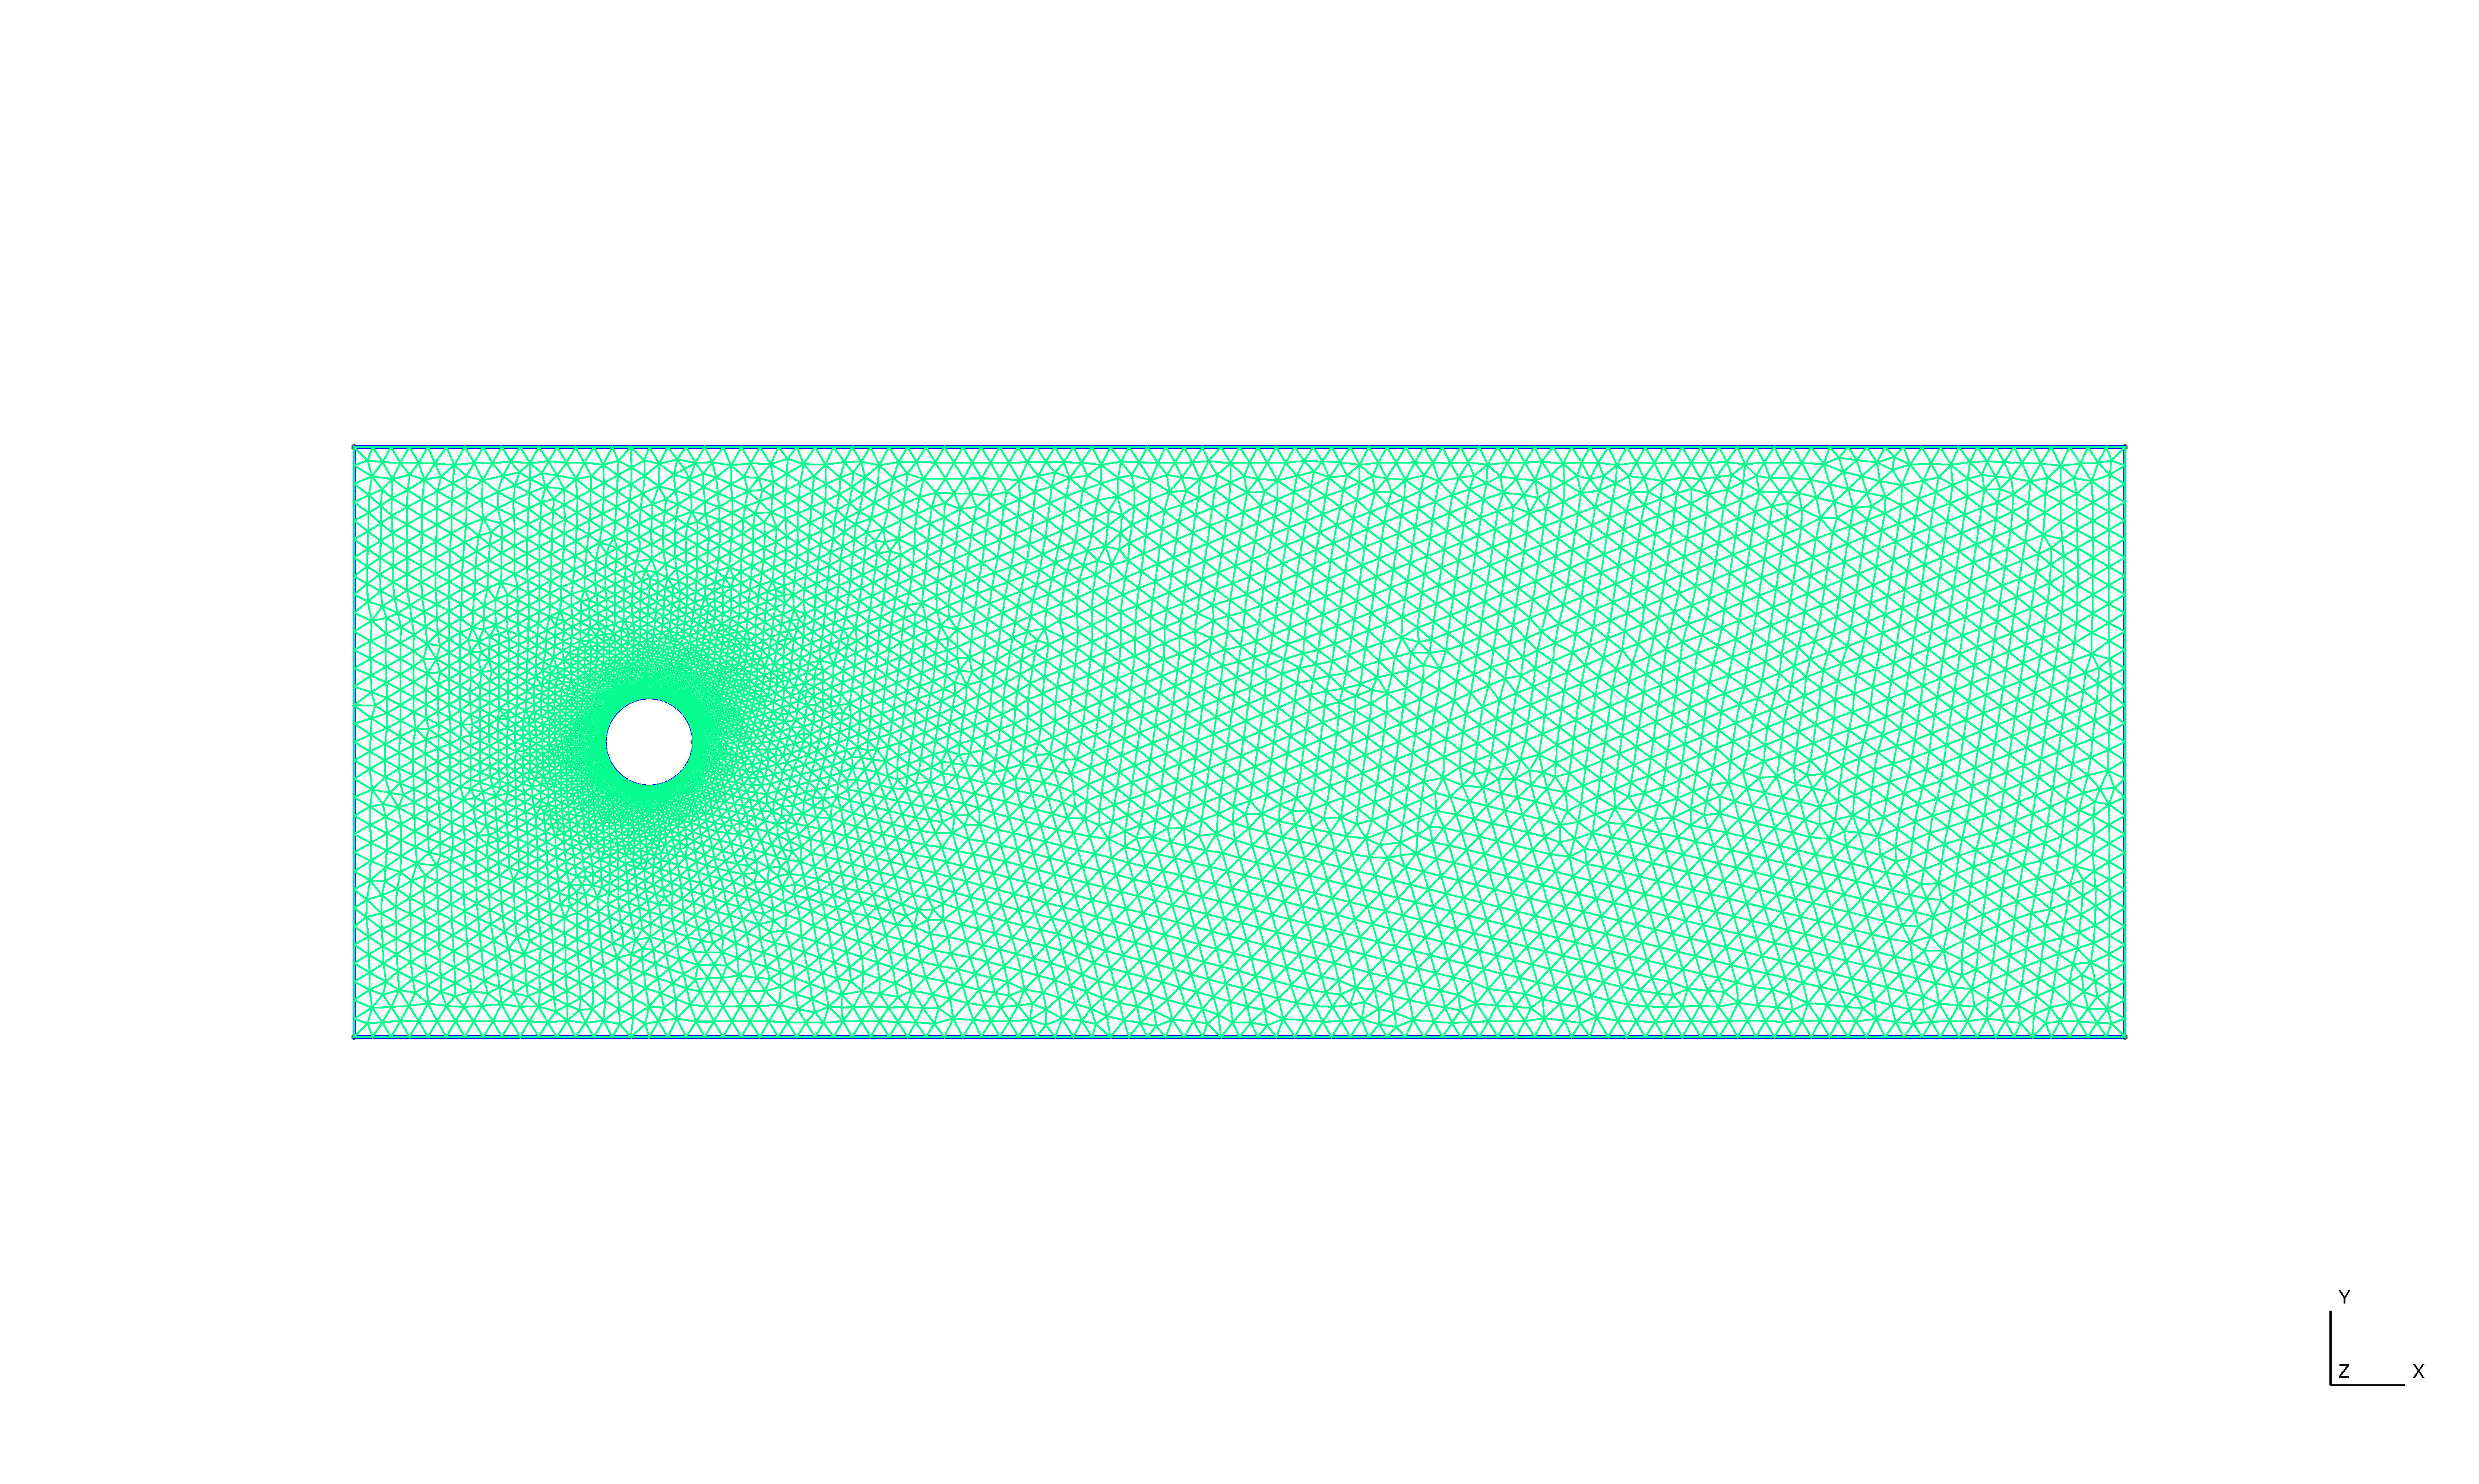
\includegraphics[width=\textwidth]{figures/mesh_domain.pdf}
  \caption{Cylinder flow domain.}
  \label{fig:domain}
\end{figure}

The rectangular domain spans the space $\left[0,6\right]\times\left[0,2\right]\in\mathbb{R}^2$.  The cylindrical hole is centered at the point $\left(1,1\right)$ and has radius of $0.15$.  This problem has an effective Reynolds number of 62.5, which is conducive to creating vortex shedding (Fig \ref{fig:vortex}).
\begin{figure}[h]
  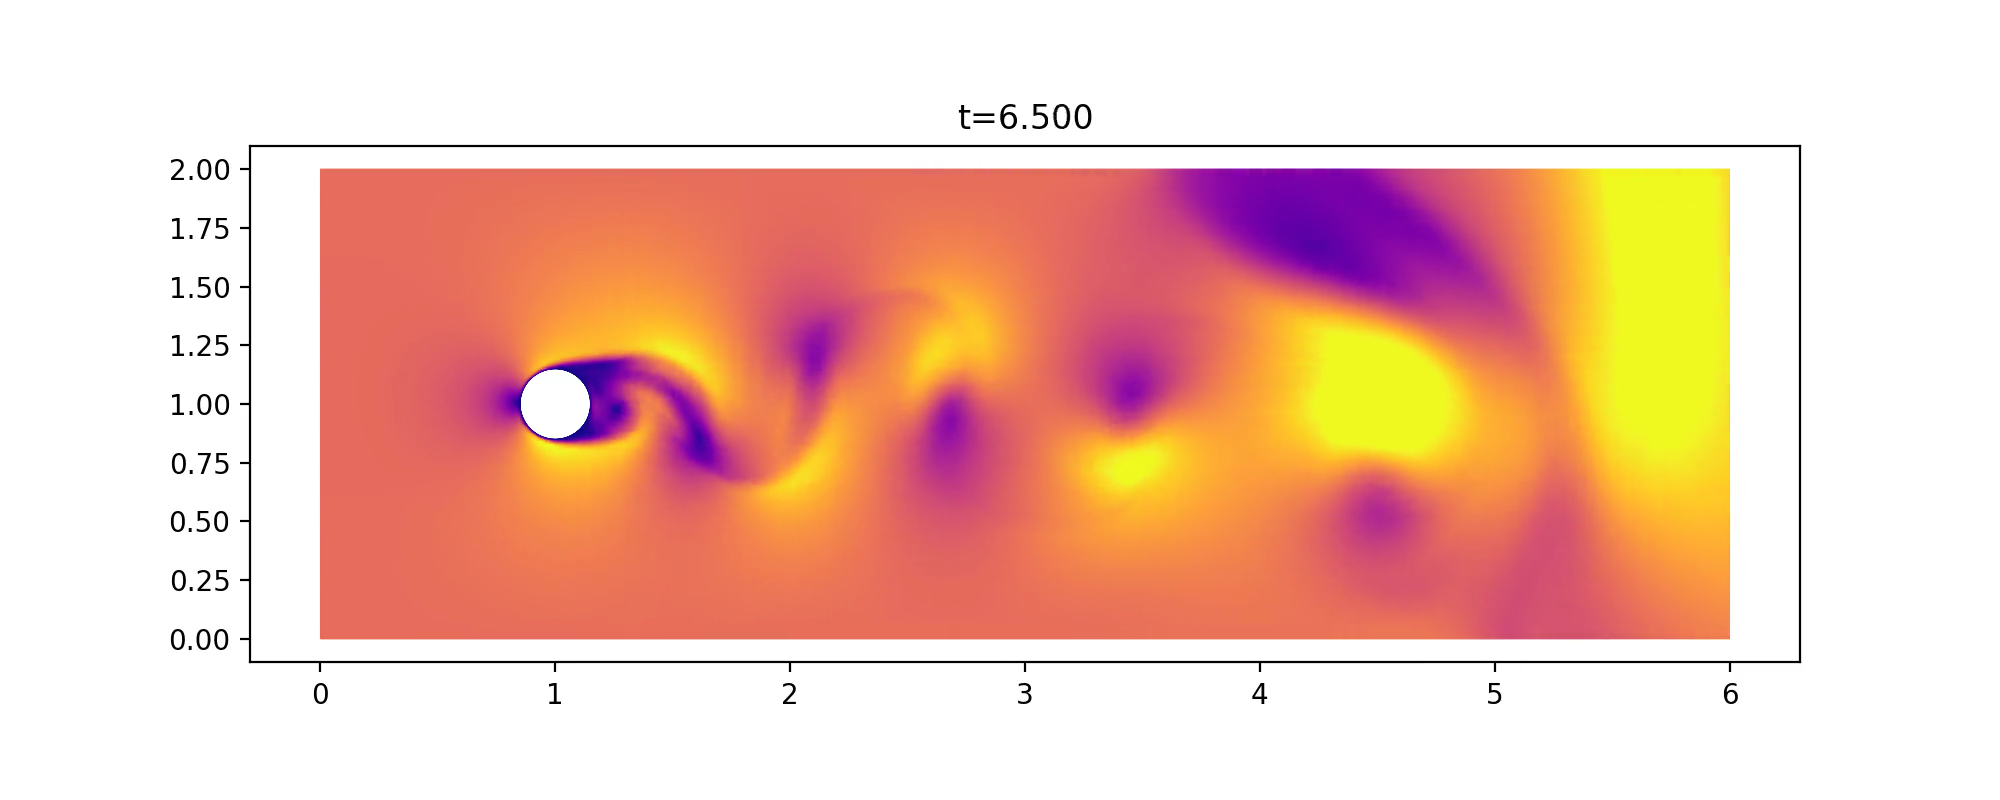
\includegraphics[width=\textwidth]{figures/vortex.png}
  \caption{Solution to the problem at $t=6.5$.  Note the vortex shedding phenomena that is visible to the right of the cylinder.}
  \label{fig:vortex}
\end{figure}

\section{Firedrake Solver}
The Firedrake\cite{Firedrake} solution to the above problem uses a ``Flexible'' GMRES KSP solver to solve the overall linearized system -- \textit{flexible} in that the preconditioner is allowed to change between iterations.  This is preconditioned by a PETSc fieldsplit PC, allowing the velocity and pressure blocks to be separately solved.

The velocity block is solved using an AMG-preconditioned GMRES solver.  The AMG routine is a Ruge-St\"uben solver courtesy of PyAMG\cite{OlSc2018}.

The pressure Schur complement is solved using a time-dependent PCD preconditioner as outlined in \eqref{eqn:pcdrfinal}.  This is a slight modification of the PCD preconditioner that is built-in to Firedrake itself.  Each of the sub-matrices in the PCD preconditioner (pressure laplacian, pressure mass, and reaction compnent) are solved using a direct LU solver.

\section{Learning Interpolation}
Below are a few ideas on how to effectively learn an AMG interpolation operator for the above Navier-Stokes problem.  These can be considered an extension of the techniques presented by Luz, Galun, Maron, Basri, and Yavneh \cite{luz2020learning} and follow the classical AMG setup of first creating the C/F partitioning and the interpolation operator itself.  The basic method is to have two separate graph networks working serially:
\begin{enumerate}
\item A first graph network that, for a given A matrix, will output an optimal C/F partitioning for the problem.  The output should be a vector $\vec{c}$ whose entries lie in the range $\left[0,1\right]$ where $0$ corresponds to fine points and $1$ to coarse points.  Denote this as the \textit{P-network}.
\item Another graph network that takes a C/F partitioning and outputs the columns of the interpolation operator $\mat{P}$.  If necessary, the graph edge data could be used to impose a sparsity pattern on the resultant columns.  Denote this as the \textit{CF-network}.
\end{enumerate}

Having the two ``steps'' as separate networks can bring a few benefits.  One is that each network could be trained separately and then combined later to create a full AMG method -- each having a different loss function, training set, etc.
\subsection{Loss Function}
To train the networks, we will use a loss function based on the spectral radius of the error propagator:
\begin{equation}
  \mat{E} := \mat{R}^\nu \mat{C} \mat{R}^\nu
\end{equation}
where $\mat{R}$ is the error propagation per iteration of the relaxation scheme, $\nu$ is the number of pre-and-post-relaxation steps, and $\mat{G}$ is the coarse-grid correction error propagator,
\begin{equation}
  \mat{G} := \mat{I} - \mat{P} \left( \mat{P}^T \mat{A} \mat{P} \right)^{-1} \mat{P}^T \mat{A}.
\end{equation}
In this case, weighted Jacobi iteration is used for the relaxation scheme with a weight of $\omega=\frac{2}{3}$, giving an error propagator of
\begin{equation}
  \mat{R} := \mat{I} - \frac{2}{3}\mat{D}^{-1}\mat{A},
\end{equation}
where $\mat{D}=\text{diag}\left(\mat{A}\right)$.  In theory, an optimal interpolation operator should minimize the spectral radius of the error propagator, $\rho\left(\mat{E}\right)$.  However, backpropagation of the maximal eigenvector computed through, power iteration for example, tends to be rather unstable and can lead to numerical overflow\cite{wang2019backpropagationfriendly}.  Therefore, as proposed in \cite{luz2020learning}, minimizing the squared Frobenius norm, $\norm{\mat{A}}_F^2=\sum\lambda^2_i\left(\mat{A}\right)$ for SPD $\mat{A}$ can be done as a proxy.

Using purely the error propagator as the loss will simply minimize the number coarse points in the final interpolation operator, which is unwanted.  Therefore, we will want to add a penalty proportional to the number of coarse points.  If we allow $\vec{c}$ to be the vector containing the C/F splitting and whose entries float between $0$ (fine) and $1$ (coarse), we can use the $L_1$ norm $\norm{\vec{c}}_1$ to penalize how ``dense'' the vector is.

Bringing this all together, we obtain the final loss function
\begin{equation}
  \ell := \norm{\mat{E}}^2_F + \alpha \norm{\vec{c}}_1^2 \label{eqn:loss}
\end{equation}
for some scaling coefficient $\alpha$.

There still remains the question of how do we represent the interchange of data between the ``CF'' network and the ``P'' network?  If we were to discretely split the C/F space at 0.5, and for example take $c_i\geq 0.5$ to be coarse points and $c_i<0.5$ to be fine points, we would run into the issue of having a discontinuous loss function in that gradient-descent based methods could not effectively train our pair of networks.   If our points are \textit{either} coarse \textit{or} fine, will we have any gradient information that would allow us to switch assignments?

After some discussion with Matt, a few possible strategies are outlined below.
\subsubsection{Continuous Loss}
In this stategy, instead of generating $\mat{P} \in \mathbb{R}^{N_F\times N_C}$, we instead generate the ``full'' operator $\hat{\mat{P}} \in \mathbb{R}^{N_F \times N_F}$.  I.e., we compute all columns of the interpolation operator as if each node was coarse.  Let $\mat{C} := \text{diag}\left(\vec{c}\right)$, then we can update the coarse-grid propagator by somehow replacing $\mat{P}$ with $\hat{\mat{P}}$ and $\mat{C}$:
\begin{equation}
  \mat{G} := \mat{I} - \mat{P} \left( \mat{P}^T \mat{A} \mat{P} \right)^{-1} \mat{P}^T \mat{A}.
\end{equation}
I don't know.  Matt and I got kind of stuck here.  Matt suggested
\begin{equation}
  \mat{P} = \mat{C} \hat{\mat{P}} \mat{C} + \left(\mat{I} - \mat{C}\right),
\end{equation}
effectively inserting zeros into the columns of $\hat{\mat{P}}$ then replacing them with $1$.  The idea here is to find \textit{``some way to stick $\text{diag}\left(\vec{c}\right)$ into the calculation of $\mat{E}$ in a way that, if $\vec{c}$ is just $0$s and $1$s we get exactly the right $\mat{E}$''.}
\subsubsection{Reinforcement Learning, ``Generalized Ali Method''}
Here, we reframe the problem into a RL context.  Training is initialized with a partitioning of only fine points, then after each training step some node is flipped from fine to coarse according to the following algorithm:
\begin{enumerate}
\item For timestep $t$, let $\hat{\mat{P}}_t$ and $\mat{c}_t$ be the interpolation and c/f splitting, respectively.
\item Have an RL network that takes $\hat{\mat{P}}_t$, $\mat{c}_t$, outputs $\widetilde{\mat{P}}_t$, $\widetilde{\mat{c}}_t$.
\item Take the largest entry in $\widetilde{\vec{c}}_t - \vec{c}_t$ as an indicator of needing to flip entry $i$ from fine to coarse.  Generate $\hat{\mat{P}}_{t+1}$ and $\mat{c}_{t+1}$ from this new information.
\item Repeat until some specified stopping condition.
\end{enumerate}
At each timestep, we can directly use the discontinuous loss from \eqref{eqn:loss}.
\subsubsection{Reinforcement Learning, ``Generalized AlphaGo Method''}
Use MCTS like AlphaGo.  This would have the benefit of having another network that could out some measure of ``goodness'' for a given interpolation operator.  This could be helpful in answering the research question in the introduction: can we reuse AMG setups for multiple timesteps until we can confidently \textit{guess} that they will no longer be effective?

I don't have a lot to say about this one.  I would need to do some reading about this.
\subsubsection{Hybrid RL and Unsupervised Method, ``Ali + Nicolas Method''}
Here, we decouple the \textit{P-net} and \textit{CF-net} networks and learn the former by an RL method and the latter by some unsupervised loss.  The training algorithm would follow this outline:
\begin{enumerate}
\item First, train the \textit{P-net} on various randomly-generated CF partitions.  Here, we would only use the squared Frobenius norm, $\norm{\mat{E}}_F^2$, as the loss.
\item Now, train the \textit{CF-net} as in the \textit{Generalized Ali Method} using the loss function $\ell := \norm{\mat{E}\left(P\left(\vec{c}\right)\right)}_F^2 + \alpha\norm{\vec{c}}_1$, where the $\mat{E}\left(P\left(\vec{c}\right)\right)$ refers to the error propagator of the interpolation operator generated from coarsening $\vec{c}$ by the \textit{P-net}.
\item After each episode of RL training, train the \textit{P-net} on the coarsenings generated by the \textit{CF-net} so that the \textit{P-net} can learn to effectively generate interpolations for the coarsenings we find.
\item Repeat steps $(2)$ and $(3)$ until some specified stopping condition.
\end{enumerate}
\nocite{*}
\bibliographystyle{siam}
\bibliography{navier}
\end{document}
